\section{Comparison}
This section presents the results of the comparison of the heuristic methods presented in Section~\ref{Section:theory}.
While the heuristics were compared on thousands of problems, only the results of four are presented in this protocol due to trade secrets.
Specifically, the methods were compared across four real-life scheduling problems obtained from a data-processing engine.
The problems contained between 7 and 12 activities, and the resources corresponded to the number of CPU cores available to the engine.
One problem was presented in Section~\ref{Section:theory}, and three problems are presented in this section.

For each problem, the CPM network is presented.
In this section, the edges representing jobs in the CPM networks have two values associated with them: computation time in seconds and CPU cores required.

\subsection{Problem 1}
The visualization of problem 1 as a CPM network is shown in Figure~\ref{Figure:comparion->problem->1->cpm-network}. For this problem, $r_\mathrm{max}$ was set to 7.

\begin{figure}[ht!]
	\centering
	\begin{tikzpicture}[
		mynode/.style={
			circle,
			draw=black,
			fill=gray,
			fill opacity = 0.3,
			text opacity=1,
			inner sep=0pt,
			minimum size=20pt,
			font=\small},
		myarrow/.style={-Stealth},
		node distance=0.6cm and 1.2cm
		]
		\node[mynode] (n1) {1};
		\node[mynode,above right=of n1] (n2) {2};
		\node[mynode,below=of n2] (n3) {3};
		\node[mynode,below=of n3] (n4) {4};
		\node[mynode,right=of n3] (n5) {5};
		\node[mynode,right=of n5] (n6) {6};
		
		\foreach \i/\j/\txt/\p in {% start node/end node/text/position
			n1/n2/{4, 3}/above,
			n1/n3/{6, 5}/above,
			n1/n4/{5, 4}/above,
			n2/n5/{3, 3}/above,
			n3/n5/{4, 3}/above,
			n4/n6/{4, 5}/below,
			n5/n6/{3, 3}/above}
		\draw [myarrow] (\i) -- node[sloped,font=\small,\p] {\txt} (\j);
		
	\end{tikzpicture}
	\caption{Visualization of problem 1 as a CPM network.
		Each weighted edge represents a job, its duration (in seconds), and the number of CPU cores required.
	}
	\label{Figure:comparion->problem->1->cpm-network}
\end{figure}

The timelines produced by SHM, PHM, and PHMDP are shown in Figures~\ref{Figure:comparison->problem->1->timelines->shm}, \ref{Figure:comparison->problem->1->timelines->phm}, and \ref{Figure:comparison->problem->1->timelines->phmdp}, respectively.
As can be seen from the figure, unexpectedly, PHM produced the best results for this problem as it scheduled the jobs to be completed within 20 seconds.
However, PHMDP was only one second behind.
This is due to the dynamic priorities holding back certain jobs, such as 1-4, even though they need not have been.

\begin{figure}[ht!]
	\centering
	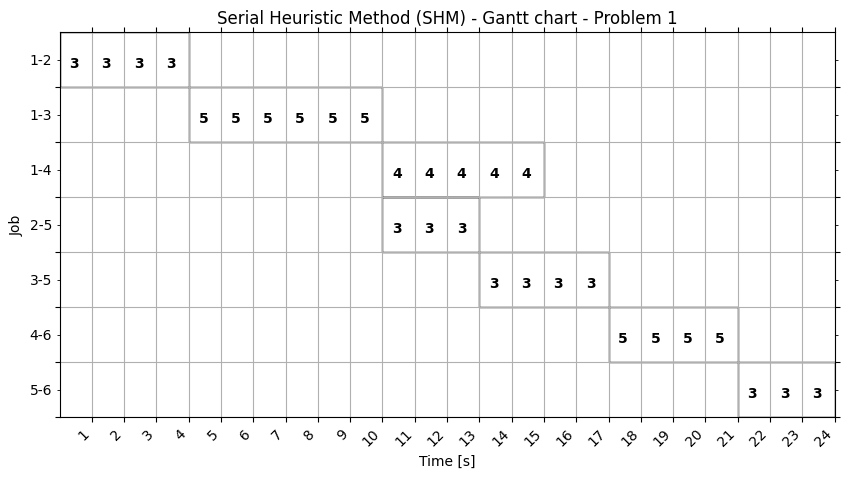
\includegraphics[width=0.7\linewidth]{images/comparison/shm_problem_1.png}
	\caption{Timeline of the activities in problem 1 as scheduled by SHM.
		The vertical axis represents the job, while the horizontal axis displays the time in seconds.
		The numbers in the squares represent the CPU cores required by each job at a point in time.
	}
	\label{Figure:comparison->problem->1->timelines->shm}
\end{figure}

\begin{figure}[ht!]
	\centering
	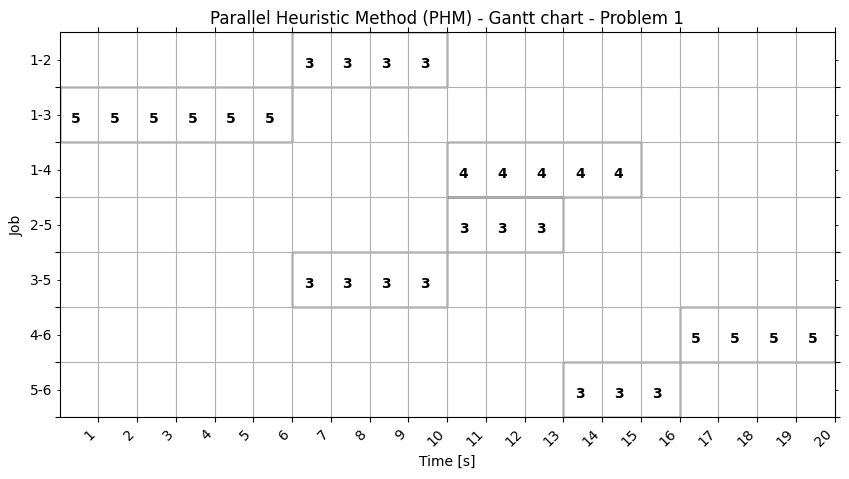
\includegraphics[width=0.7\linewidth]{images/comparison/phm_problem_1.png}
	\caption{Timeline of the activities in problem 1 as scheduled by PHM.}
	\label{Figure:comparison->problem->1->timelines->phm}
\end{figure}

\begin{figure}[ht!]
	\centering
	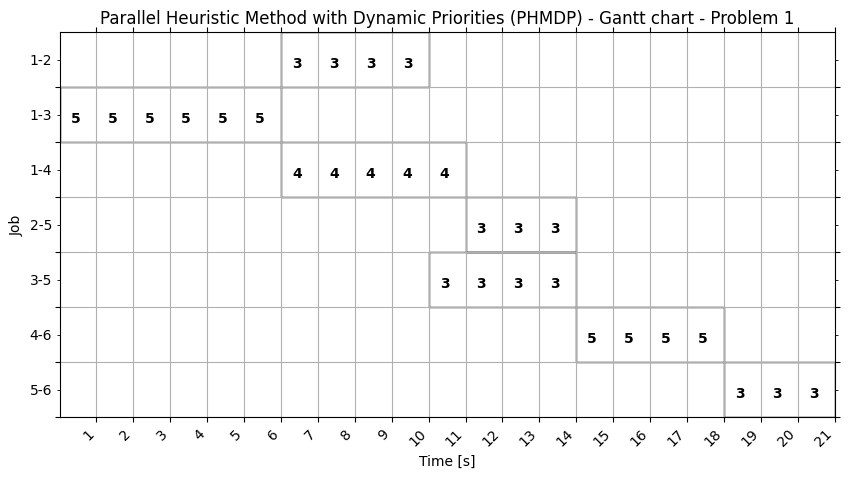
\includegraphics[width=0.7\linewidth]{images/comparison/phmdp_problem_1.png}
	\caption{Timeline of the activities in problem 1 as scheduled by PHMDP.}
	\label{Figure:comparison->problem->1->timelines->phmdp}
\end{figure}

\subsection{Problem 2}
The visualization of problem 2 as a CPM network is shown in Figure~\ref{Figure:comparion->problem->2->cpm-network}. For this problem, $r_\mathrm{max}$ was set to 8.

\begin{figure}[ht!]
	\centering
	\begin{tikzpicture}[
		mynode/.style={
			circle,
			draw=black,
			fill=gray,
			fill opacity = 0.3,
			text opacity=1,
			inner sep=0pt,
			minimum size=20pt,
			font=\small},
		myarrow/.style={-Stealth},
		node distance=0.6cm and 1.2cm
		]
		\node[mynode] (n1) {1};
		\node[mynode,above right=of n1] (n2) {2};
		\node[mynode,below right=of n1] (n3) {3};
		\node[mynode,below right=of n2] (n4) {4};
		\node[mynode,above right=of n4] (n5) {5};
		\node[mynode,below right=of n4] (n6) {6};
		\node[mynode,below right=of n5] (n7) {7};
		
		\foreach \i/\j/\txt/\p in {% start node/end node/text/position
			n1/n2/{5, 3}/above,
			n1/n3/{6, 4}/above,
			n1/n4/{10, 3}/above,
			n2/n4/{1, 3}/above,
			n2/n5/{6, 2}/above,
			n3/n4/{2, 3}/above,
			n3/n6/{5, 3}/above,
			n4/n5/{8, 3}/below,
			n4/n6/{7, 2}/below,
			n5/n6/{9, 4}/above,
			n5/n7/{7, 4}/above,
			n6/n7/{12, 4}/above}
		\draw [myarrow] (\i) -- node[sloped,font=\small,\p] {\txt} (\j);
		
	\end{tikzpicture}
	\caption{Visualization of problem 2 as a CPM network.
		Each weighted edge represents a job, its duration (in seconds), and the number of CPU cores required.
	}
	\label{Figure:comparion->problem->2->cpm-network}
\end{figure}

The timelines produced by SHM, PHM, and PHMDP are shown in Figures~\ref{Figure:comparison->problem->2->timelines->shm}, \ref{Figure:comparison->problem->2->timelines->phm}, and \ref{Figure:comparison->problem->2->timelines->phmdp}, respectively.
In the case of problem 2, PHMDP scheduled the jobs to be completed in the shortest time: 41 seconds.
However, the slowest heuristic, SHM, was only three seconds behind.

\begin{figure}[ht!]
	\centering
	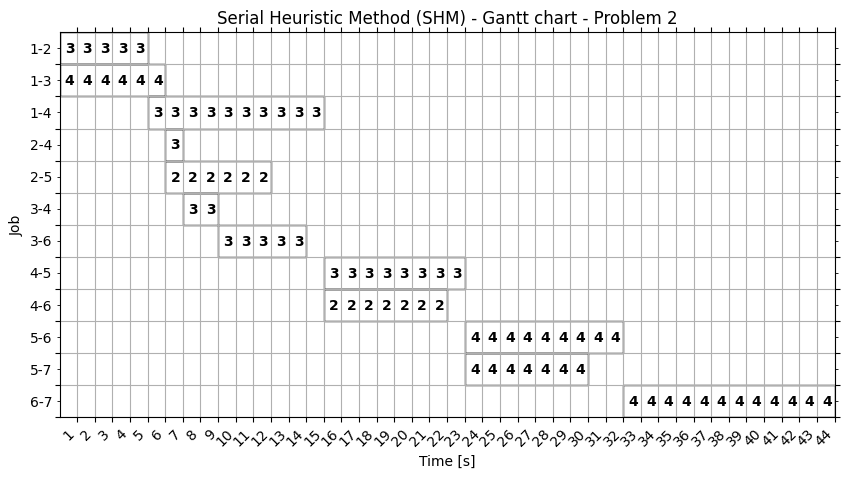
\includegraphics[width=0.8\linewidth]{images/comparison/shm_problem_2.png}
	\caption{Timeline of the activities in problem 2 as scheduled by SHM.
		The vertical axis represents the job, while the horizontal axis displays the time in seconds.
		The numbers in the squares represent the CPU cores required by each job at a point in time.
	}
	\label{Figure:comparison->problem->2->timelines->shm}
\end{figure}

\begin{figure}[ht!]
	\centering
	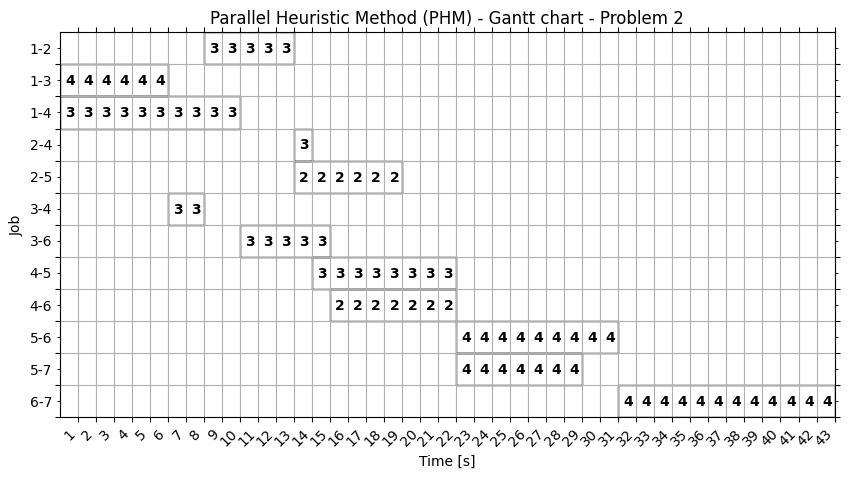
\includegraphics[width=0.8\linewidth]{images/comparison/phm_problem_2.png}
	\caption{Timeline of the activities in problem 2 as scheduled by PHM.}
	\label{Figure:comparison->problem->2->timelines->phm}
\end{figure}

\begin{figure}[ht!]
	\centering
	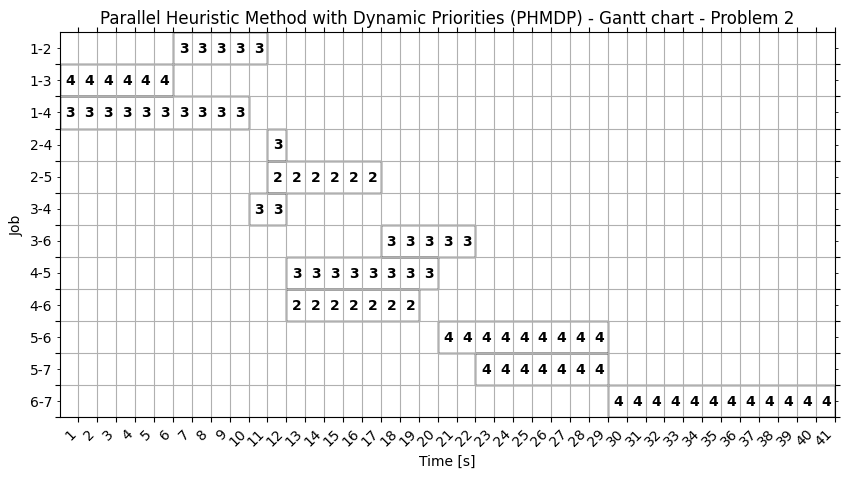
\includegraphics[width=0.8\linewidth]{images/comparison/phmdp_problem_2.png}
	\caption{Timeline of the activities in problem 2 as scheduled by PHMDP.}
	\label{Figure:comparison->problem->2->timelines->phmdp}
\end{figure}

\subsection{Problem 3}
The visualization of problem 3 as a CPM network is shown in Figure~\ref{Figure:comparion->problem->3->cpm-network}. For this problem, $r_\mathrm{max}$ was set to 6.

\begin{figure}[ht!]
	\centering
	\begin{tikzpicture}[
		mynode/.style={
			circle,
			draw=black,
			fill=gray,
			fill opacity = 0.3,
			text opacity=1,
			inner sep=0pt,
			minimum size=20pt,
			font=\small},
		myarrow/.style={-Stealth},
		node distance=0.6cm and 1.2cm
		]
		\node[mynode] (n1) {1};
		\node[mynode,above right=of n1] (n2) {2};
		\node[mynode,below=of n2] (n3) {3};
		\node[mynode,below=of n3] (n4) {4};
		\node[mynode,right=of n2] (n5) {5};
		\node[mynode,right=of n5] (n7) {7};
		\node[mynode,below=of n7] (n6) {6};
		
		
		\foreach \i/\j/\txt/\p in {% start node/end node/text/position
			n1/n2/{4, 3}/above,
			n1/n3/{3, 4}/above,
			n1/n4/{5, 3}/above,
			n2/n5/{3, 2}/above,
			n3/n5/{2, 3}/above,
			n4/n6/{4, 2}/below,
			n5/n6/{3, 4}/above,
			n5/n7/{4, 3}/above}
		\draw [myarrow] (\i) -- node[sloped,font=\small,\p] {\txt} (\j);
		
	\end{tikzpicture}
	\caption{Visualization of problem 3 as a CPM network.
		Each weighted edge represents a job, its duration (in seconds), and the number of CPU cores required.
	}
	\label{Figure:comparion->problem->3->cpm-network}
\end{figure}

The timelines produced by SHM, PHM, and PHMDP are shown in Figures~\ref{Figure:comparison->problem->3->timelines->shm}, \ref{Figure:comparison->problem->3->timelines->phm}, and \ref{Figure:comparison->problem->3->timelines->phmdp}, respectively.
In the case of problem 3, PHM and PHDMP tied in scheduling the jobs to complete in the shortest time: 17 seconds.
However, SHM was only two seconds behind.

\begin{figure}[ht!]
	\centering
	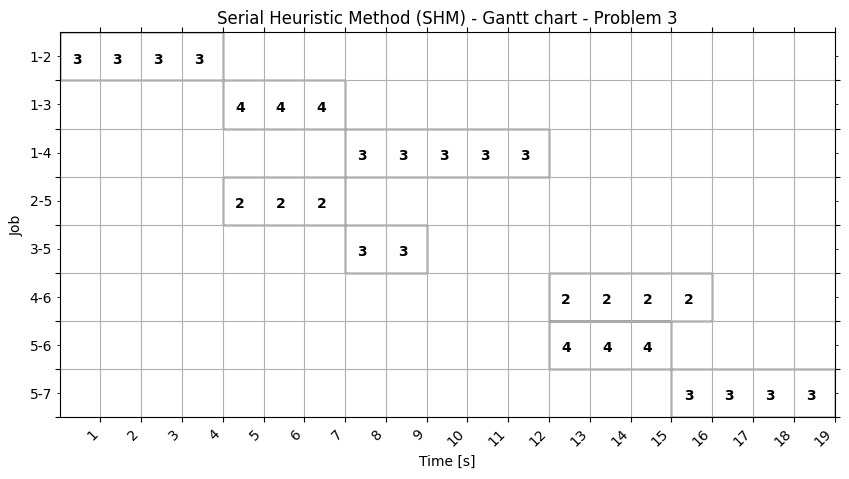
\includegraphics[width=0.8\linewidth]{images/comparison/shm_problem_3.png}
	\caption{Timeline of the activities in problem 3 as scheduled by SHM.
		The vertical axis represents the job, while the horizontal axis displays the time in seconds.
		The numbers in the squares represent the CPU cores required by each job at a point in time.
	}
	\label{Figure:comparison->problem->3->timelines->shm}
\end{figure}

\begin{figure}[ht!]
	\centering
	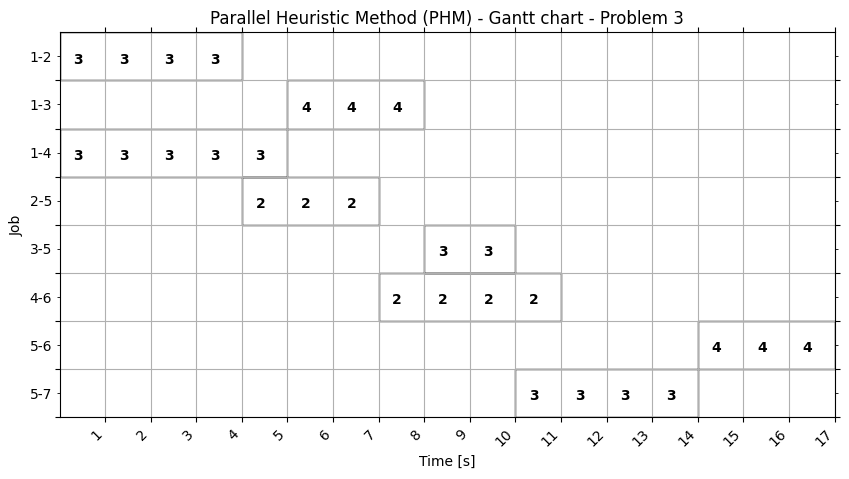
\includegraphics[width=0.8\linewidth]{images/comparison/phm_problem_3.png}
	\caption{Timeline of the activities in problem 3 as scheduled by PHM.}
	\label{Figure:comparison->problem->3->timelines->phm}
\end{figure}

\begin{figure}[ht!]
	\centering
	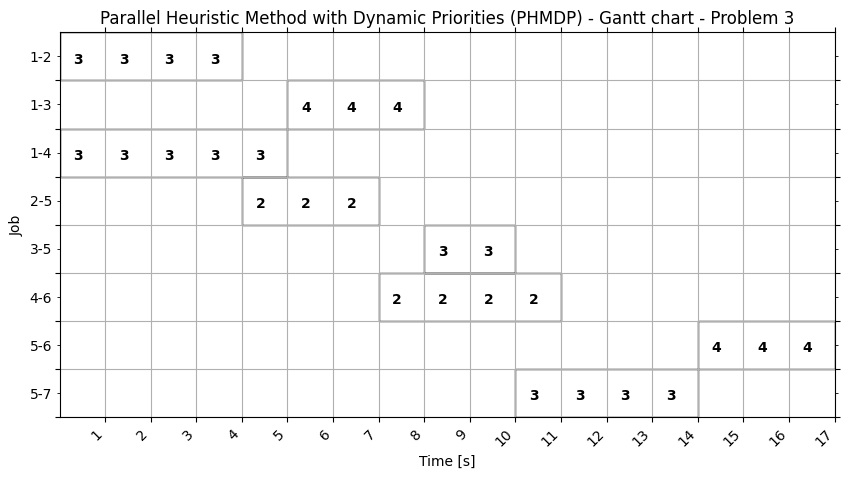
\includegraphics[width=0.8\linewidth]{images/comparison/phmdp_problem_3.png}
	\caption{Timeline of the activities in problem 3 as scheduled by PHMDP.}
	\label{Figure:comparison->problem->3->timelines->phmdp}
\end{figure}